% Contributors: William Tong, Will Zheng
\section{Variations on a Theme of DBSCAN}

With an algorithm as old and widely adopted as DBSCAN, many have dedicated considerable energy towards improving the method. Common themes have included accelerating the runtime, improving robustness, alleviating sensitivity to parameters, and discovering clusters of varying densities. To give a flavor of the breadth, some examples are:\cite{dbscan_improvs}

\begin{itemize}
    \item \textbf{GDBSCAN} (Generalized DBSCAN): generalizes the algorithm to non-Euclidean spaces, for example general metric spaces
    \item \textbf{ST-DBSCAN} (Spatial-Temporal DBSCAN): considers an added time dimension when clustering
    \item \textbf{DVBSCAN} (Density Variation Based Spatial Clustering of Applications with Noise): addresses local density variation within a cluster, allowing decent performance on clusters with non-uniform density
    \item \textbf{MR-DBSCAN} (MapReduce DBSCAN): uses the popular big data algorithm to speed computation; also addresses clusters with uneven density distribution
    \item \textbf{HDBSCAN\textsuperscript{*}} (Hierarchical DBSCAN): extends DBSCAN to extract hierarchical clusters
    \item \textbf{PACA-DBSCAN} (Polymorphic Ant Colony Algorithm DBSCAN): applies ant colony optimization (ACO) techniques to aid clustering in higher dimensions. ACOs reduce the problem to a graph traversal setting, finding an optimal path through exploration methods inspired by ants.
\end{itemize}

In the following sections, we will focus particularly on two improvements that have substantial potential or success: DBSCAN++ and OPTICS \\

\noindent\textbf{DBSCAN++}

The worse-case runtime of a classic DBSCAN implementation is $O(n^2)$. In practice, with clever indexing and relatively well-behaved data, the runtime is closer to $O(n \log(n))$. But the threat of quadratic runtime remains a real problem, especially in a world of big data.

The goal of DBSCAN++ is to achieve sub-quadratic runtime while maintaining good levels of performance. It does so by sampling only a proportion of the total data when checking for core points, then generating clusters based only on the discovered cores. See below for the formal algorithm.\cite{dbscanpp}

  \begin{algorithm}[H]
    \caption{DBSCAN++ Algorithm}
    \label{dbscan++ alg}
    \begin{algorithmic}[1]
      \renewcommand\algorithmicrequire{\textbf{input}}
      \REQUIRE $X = {x_1\cdots x_n}$, $\epsilon \in \bbR^+$, $m \in \bbN^*$
      \STATE Sample $S \subset X$
      \STATE Let $C=\{x \in S \ | \ X \cap B(x, \epsilon) \geq m\}$.
      \STATE Construct the graph $G=(V,E)$, with $V=C$, $E=\{(i,j) \ | \ ||x_i-x_j|| \leq \epsilon\}$.
      \STATE Run connected components on $G$. The clusters are the connected components.
      \STATE Let $B=\{x \in X \ | \ x \notin C, \exists c \in C, ||x-c|| \leq \epsilon\}$.
      For each $b \in B$, assign $b$ to the connected component of any arbitrary $c \in C$
      that is within $\epsilon$ of $b$.
      \STATE Ignore the rest of the points, which we consider noise points.
    \end{algorithmic}
  \end{algorithm}
  
Hence instead of iterating over all points to discover cores, we iterate over a subset $S$. The cluster queries then occur only for core points within the subset, reducing the overall runtime to $O(sn)$, where $s = |S| < n$. In fact, under reasonable regularity conditions, it can be shown that the runtime can be subquadratic:

$$ O(n^{2 - 2\beta / (2\beta + D})$$
where $D$ is the number of dimensions and $\beta$ is a positive constant representing a smoothness assumption placed on the density level sets (elaborated below in the description of Robust DBSCAN). The bound is achieved when $|S|$ is roughly greater than $n^{D / (2\beta + D)}$, on a dataset with $n$ points. Note that a higher $\beta$ corresponds to a "smoother" dataset, where the differences in density are harder to discern, resulting in a smaller number of larger clusters. The chance of a random sample including core points from a cluster rises. This effect is reflected in the runtime, in which a higher $\beta$ yields a faster runtime. On the other hand, higher dimensional data implies sampling more points to cover the space. So as the $D$ increases, the algorithm naturally slows.

See Figure \ref{fig:runtime} for a direct comparison of runtimes.

\begin{figure}[h]
\centering
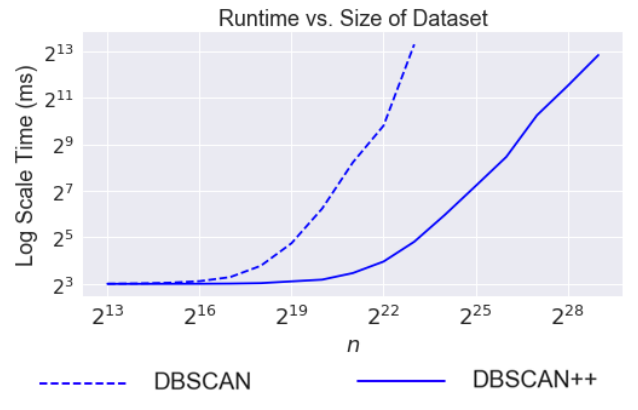
\includegraphics[scale=0.48]{chapter_2/files/dbscan_plus_runtimes.png}
\caption{Data was generated from a three dimensional Guassian mixture with four components. Observe that DBSCAN begins to exhibit quadratic behavior after $n=2^19$. Source: \cite{dbscanpp}}
\label{fig:runtime}
\end{figure}

There are two main methods for sampling the dataset:
\begin{enumerate}
    \item \textbf{Uniform}: random uniform sample across all data points
    \item \textbf{K-Center}: greedy furthest-first traversal approximation to the K-Center problem applied to the dataset, where $k$ is the number of elements in the sample
\end{enumerate}

Both methods have the same consistency guarantees for approximating the density in a dataset. But in practice, the K-Center approach may yield a more even spread of samples than uniform sampling, potentially contributing to better result (see Figures \ref{fig:dbscan_plus} and \ref{fig:dbscan_plus_scores}).

\begin{figure}[h]
\centering
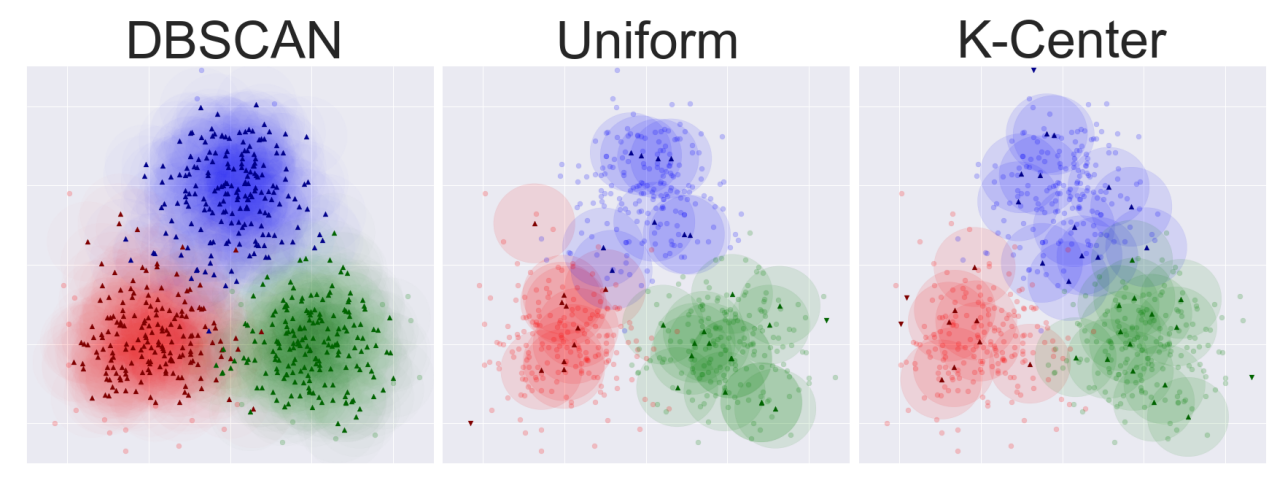
\includegraphics[scale=0.27]{chapter_2/files/dbscan_plus_comparison.png}
\caption{A comparison of DBSCAN++ sampling methods with traditional DBSCAN clustering. Performance is fairly consistent across the three examples, with clusters discovered using K-Centers sampling perhaps slightly closer to the original than uniform sampling. Source: \cite{dbscanpp}}
\label{fig:dbscan_plus}
\end{figure}

\begin{figure}[h]
\centering
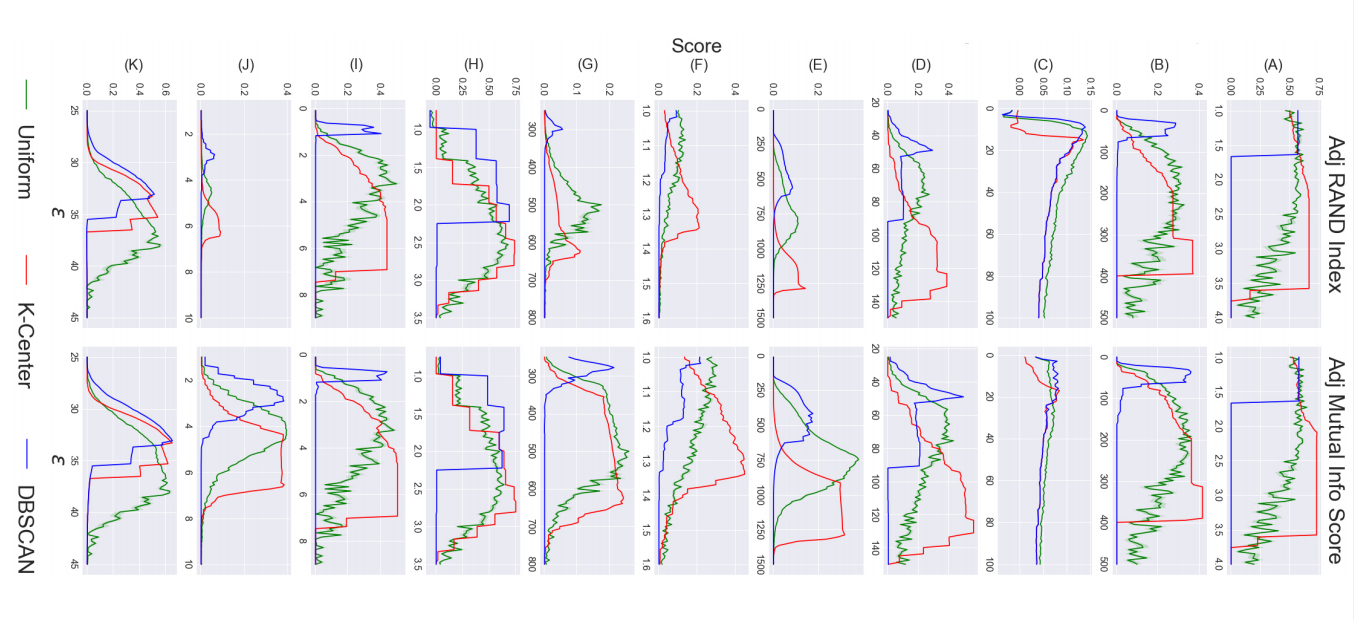
\includegraphics[scale=0.20,angle=90]{chapter_2/files/dbscan_plus_scores.png}
\caption{An empirical comparison of DBSCAN++ and DBSCAN on different datasets. Rand index and mutual information scores are generated to compare the clusters produced by DBSCANA and the two sampling methods of DBSCAN++, with varying $\epsilon$. It is apparent that DBSCAN++ is able to achieve comparable performance to DBSCAN, despite sampling a fraction of the total points. Source: \cite{dbscanpp}}
\label{fig:dbscan_plus_scores}
\end{figure}

\noindent \textbf{OPTICS}

An important issue with DBSCAN is its inability to capture clusters of varying density. Furthermore, cluster density must be manually tuned with the $\epsilon$ bandwidth parameter. Small changes in $\epsilon$ may devastate the quality of the resulting clusters.

A popular solution to both problems is OPTICS: Ordering Points To Identify the Clustering Structure. The basic setup is similar to DBSCAN, but defines two additional metrics: core distance and reachability distance. Suppose $p_{(m)}$ is the $m$th closest point to $p$. Then with $\epsilon$ bandwidth and $m$ minimum points to qualify a cluster, considering the $\epsilon$ neighborhood $N_\epsilon(P)$ of a point $p$, we define the values:

\begin{align*}
    \text{core-dist}_{\epsilon, m}(p) &= 
        \begin{cases}
            d(p, p_{(m)}) & \text{if}\; |N_\epsilon(p)| \geq m \\
            \text{undefined} & \text{otherwise} \\
        \end{cases}\\
    \text{reachability-dist}_{\epsilon, m}(p, o) &= 
        \begin{cases}
            \max \lbrace d(p, o), \text{core-dist}_{\epsilon, m} (p) \rbrace & \text{if}\; |N_\epsilon(p)| \geq m \\
            \text{undefined} & \text{otherwise} \\
        \end{cases}\\
\end{align*} \cite{wiki:optics}, \cite{medium:optics}

First, observe that both metrics apply only to core points. For border and noise points, they are undefined. Indeed, under most OPTICS implementations, border and noise points do not earn membership in any cluster, and are ignored.

\begin{figure}[h]
\centering
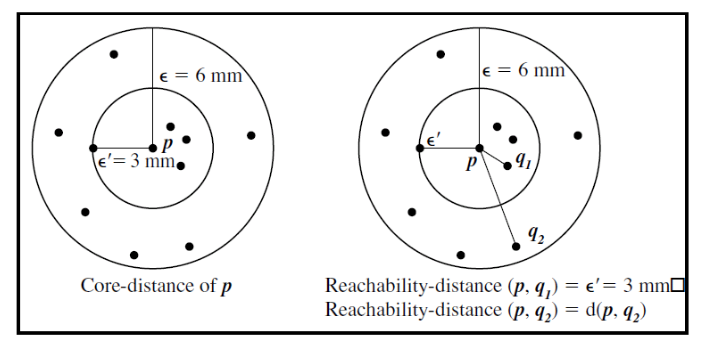
\includegraphics[scale=0.42]{chapter_2/files/optics_distances.png}
\caption{An example of core and reachability distances, from a core point $p$ and $m=4$. $\epsilon$ remains the bandwidth from the original DBSCAN algorithm. $\epsilon'$ is the core distance. Source: \cite{medium:optics}}
\label{fig:optics}
\end{figure}

Core distance is a measure of a core point's local density. If $\text{core-dist}_{\epsilon, m}(p) = \epsilon'$, then $\epsilon' << \epsilon$ implies that the core point must be in a region of high density.

Reachability distance is a measure of the distance between a core point $p$ and a nearby point $o$. In most implementations, $o$ is drawn from $N_\epsilon(p)$, in which case reachability distance will always be less than $\epsilon$. If $o$ is especially close to $p$ (i.e. within $\epsilon'$ distance of $p$), then reachability distance is the same as core distance. Otherwise, it is the actual distance between the two points.

The goal of OPTICS is to assign a reachability distance to all core points between themselves and the closest neighbor. In this way, the algorithm proceeds along a greedy shortest path traversal of the dataset, generating a reachability plot that encodes the clusters.

The algorithm proceeds as follows:

  \begin{algorithm}[H]
    \caption{OPTICS Algorithm}
    \label{optics alg}
    \begin{algorithmic}[1]
      \renewcommand\algorithmicrequire{\textbf{input}}
      \REQUIRE $X = {x_1\cdots x_n}$, $\epsilon \in \bbR^+$, $m \in \bbN^*$
      \STATE $P := \emptyset$
      \STATE $C:=\{x \in X \ | \ X \cap B(x, \epsilon) \geq m\}$.
      \STATE Update core distances for all points in $C$
      \STATE Select $p \in C$
      \WHILE{|P| < |C|}
       \STATE Select $o \in N_\epsilon (p) \setminus P$ such that $o$ minimizes $\text{reachability-dist}_{\epsilon, m}(p, o)$
       \STATE $P \leftarrow P \cup (p, d(p, o))$
       \STATE $p \leftarrow o$
      \ENDWHILE
      \RETURN $P$
    \end{algorithmic}
  \end{algorithm}
  
$P$ encodes the set of reachability distances. To produce it, we traverse the core points using lowercase point $p$, gradually performing a shortest-path traversal until all core points have been touched. The output is the set of reachability distances (along with their corresponding points) in $P$

One important quality to observe is that the bandwidth parameter $\epsilon$ has less direct impact on clustering than in traditional DBSCAN. Indeed, an $\epsilon$ large enough to cover every data point may still induce high-quality clusters, though of course runtime will suffer (worse case is $O(n^2)$). In this way, $\epsilon$ functions more like a check on the minimum density for which a cluster is interesting.

Also observe that the minimum number of points per cluster $m$ has reduced effect as well. If the value was raised, the core distances would rise accordingly, scaling all reachability distances. In this way, OPTICS is overall far less sensitive to its parameter settings than DBSCAN.  

See Figure \ref{fig:optics_plot} for an example run of OPTICS (with max $\epsilon$).

\begin{figure}[h]
\centering
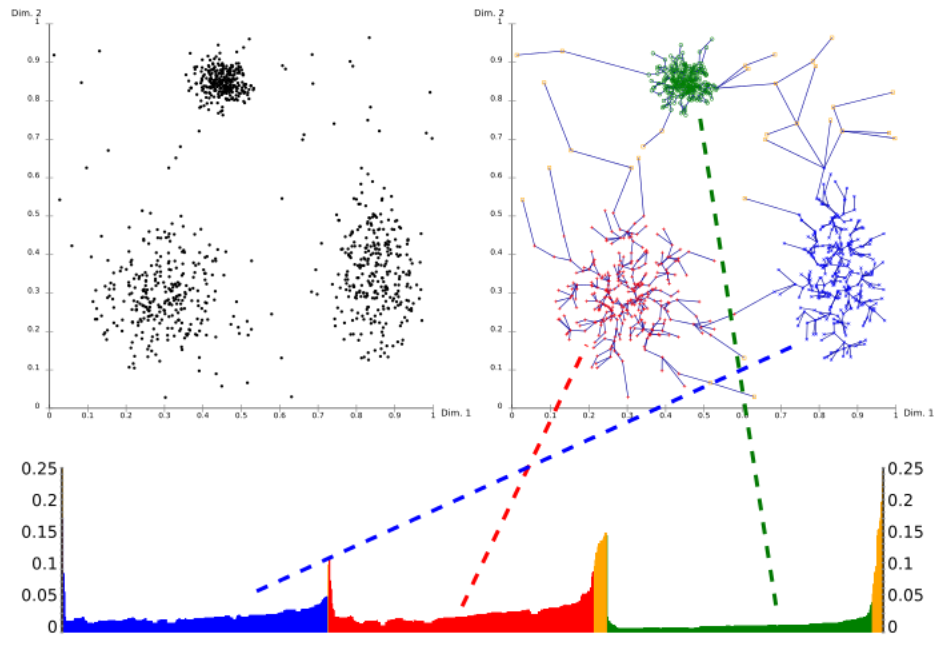
\includegraphics[scale=0.36]{chapter_2/files/optics_run.png}
\caption{An example run of OPTICS. The upper left is a plot of the dataset. The bottom shows the reachability plot. The upper right shows the resulting clusters. A separate algorithm is needed to perform postprocessing to extract the clusters. Overall, note that the varying densities of the clusters would pose a significant problem to DBSCAN. Source: \cite{wiki:optics}}
\label{fig:optics_plot}
\end{figure}

Of particular importance is the reachability plot at the bottom of the figure. The horizontal axis corresponds to the order in which the dataset was traversed, and the vertical axis the calculated reachability score. Because of the greedy shortest path traversal, points of the same cluster are also adjacent on the reachability plot. Regions of short reachability distance also appear as valleys. Denser clusters will have deeper values than sparser clusters, but the valley formation nonetheless remains intact. A separate algorithm (or manual identification) may then be used to extract the valley points as clusters, completing the process. Also note, the version of the algorithm presented has no way of addressing potential noise points in the data, but further extensions have been proposed that do provide meaningful ways of doing so (for example, see \href{https://link.springer.com/content/pdf/10.1007\%2F978-3-540-48247-5_28.pdf}{OPTICS-OF}).